\chapter{Legge di Gauss}
Consideriamo una superficie infinitesima $d \Sigma$ in una regione in cui è definito un campo $\mathbf{E}$ e orientiamola fissando il verso del versore della normale $\mathbf{u}_n$. 

Si definisce \mkeyword{flusso del campo $\mathbf{E}$}flusso del campo $\mathbf{E}$ attraverso la superficie $d\Sigma$ la quantità scalare

\begin{equation*}
    d\Phi(\mathbf{E}) = \mathbf{E} \cdot \mathbf{u}_n d\Sigma = E \cos(\theta) d \Sigma
    \label{eq:flusso_infinitesimale}
\end{equation*}

Il flusso attraverso una superficie finita $\Sigma$ si ottiene suddividendola in elementi infinitesimi di superficie $d \Sigma_i$ e sommando gli infiniti contenuti del flusso per ciascuna $i$.

\begin{figure} [h]
    \centering
    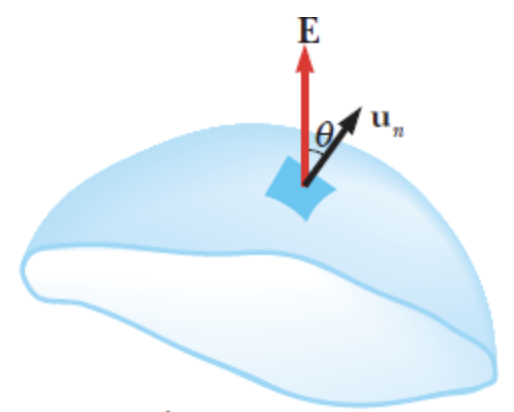
\includegraphics[width=0.4\linewidth]{figure/image6.png}
    \caption{Flusso del campo elettrico attraverso una superficie}
    \label{fig:chapter_3_1}
\end{figure}

Quindi 

\begin{equation}
    \Phi (\mathbf{E}) = \int_{\Sigma} \mathbf{E} \cdot \mathbf{u}_n d \Sigma  
\end{equation}

Se la superficie è chiusa, il flusso si scrive

\begin{equation}
    \Phi (\mathbf{E}) = \oint_{\Sigma} \mathbf{E} \cdot \mathbf{u}_n d \Sigma  
\end{equation}

Nella successiva sezione daremo la dimostrazione di una legge che si applica al campo elettrostatico, nota come \emph{legge} o teorema \emph{di Gauss}, evidenziando che questa vale \emph{se e solo se} la forza tra due cariche elementari è \emph{inversamente proporzionale al quadrato della distanza tra le stesse}.\\

La legge di Gauss \mkeyword{Legge di Gauss}afferma che il flusso del campo elettrostatico $\mathbf{E}$ prodotto da un sistema di cariche attraverso una superficie chiusa è uguale alla somma algebrica delle cariche elettriche contenute all'interno della superficie, divisa per $\varepsilon_0$

\begin{tcolorbox}[colback=yellow!10!white, colframe=orange!70!black, boxrule=0.8pt]
\begin{equation}
    \Phi(\mathbf{E}) = \oint_{\Sigma} \mathbf{E} \cdot \mathbf{u}_n \ d \Sigma = \frac{\sum_i q_i}{\varepsilon_0}
    \label{eq:Legge_di_Gauss}
\end{equation}
\end{tcolorbox}

\section{Dimostrazione della legge di Gauss}

Prima di iniziare la vera e propria dimostrazione andiamo a introdurre uno strumento che andrà a semplificare molto i calcoli, l'angolo solido.\\

Sia $d \Sigma$ un elemento di superficie, $\mathbf{u}_n$ la sua normale e $d \Sigma_0$ la sua proiezione ortogonale a $\mathbf{u}_r$, versore del raggio $r$ uscente da un punto di osservazione $O$.

\begin{figure}[h]
    \centering
    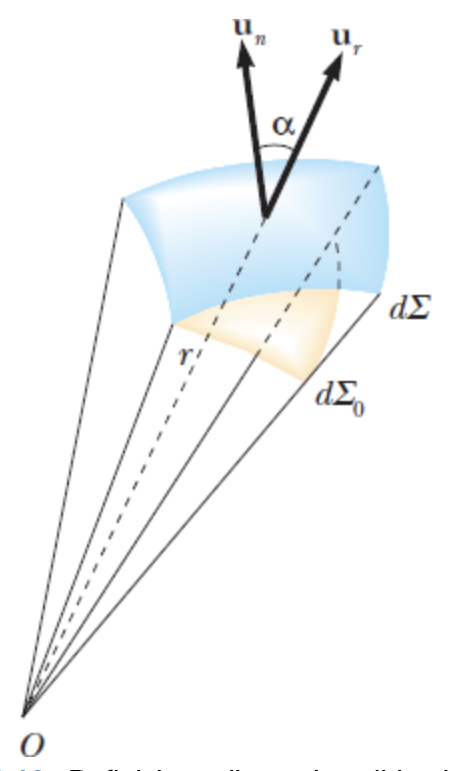
\includegraphics[width=0.32\linewidth]{figure/image7.png}
    \label{fig:chapter_3_2}
\end{figure}

Si definisce angolo solido \mkeyword{angolo solido} infinitesimo la quantità 

\begin{equation}
    d \Omega = \frac{d \Sigma \cos(\alpha)}{r^2} = \frac{d \Sigma_0}{r^2}
\end{equation}

Possiamo iniziare con la dimostrazione. Iniziamo prendendo in esame il campo elettrostatico prodotto da una carica puntiforme $q$, il flusso attraverso l'elemento di superficie orientata utilizzando la \ref{eq:flusso_infinitesimale}:

\begin{equation*}
    d \Phi(\mathbf{E}) = \frac{q}{4 \pi \varepsilon_0} \ \frac{\mathbf{u}_r \cdot \mathbf{u_n} \ d \Sigma}{r^2} = \frac{q}{4 \pi \varepsilon_0} \ \frac{d \Sigma_0}{r^2}
\end{equation*}

Per definizione $d \Sigma_0/r^2$ è l'angolo solido $d \Omega$ sotto cui è visto dalla carica $q$ il contorno di $d \Sigma$, per cui 

\begin{equation*}
    d \Phi (\mathbf{E}) = \frac{q}{4 \pi \varepsilon_0} d \Omega
\end{equation*}

Il \emph{flusso del campo elettrostatico $\mathbf{E}$ di una carica puntiforme $q$ dipende solo dall'angolo solido e non dalla superficie né dalla sua distanza dalla carica}.\\

Conviene osservare subito che la dipendenza del flusso dall'angolo solido \emph{conseguenza} del fatto che a denominatore dell'espressione del campo compare $r^2$: \emph{qualunque altra dipendenza funzionale non avrebbe portato alla \ref{eq:Legge_di_Gauss}}.\\
Il flusso attraverso una superficie finita è dato da 

\begin{equation*}
    \Phi(\mathbf{E}) = \int_{\Sigma} \mathbf{E} \cdot \mathbf{u}_n \ d \Sigma
 = \frac{q}{4 \pi \varepsilon_0} \int_{\Omega} d \Omega = \frac{q}{4 \pi \varepsilon_0} \Omega
\end{equation*}

Con $\Omega$ angolo solido sotto cui è visto il contorno della superficie $\Sigma$ dalla carica $q$.\\

Calcoliamo adesso il flusso di $\mathbf{E}$ attraverso una superficie chiusa, distinguendo due casi: quello in cui la \emph{carica $q$ è interna alla superficie} e il caso in cui è \emph{esterna}.\\

Se la carica è interna alla superficie tutti i contribuiti $\mathbf{E} \cdot \mathbf{u}_n \ d\Sigma$ si sommano in quanto hanno sempre lo stesso segno.

\begin{equation*}
    \Phi (\mathbf{E}) = \frac{q}{4\pi\varepsilon_0} \int_{\Omega} d\Omega = \frac{q}{4\pi\varepsilon_0} 4 \pi = \frac{q}{\varepsilon_0}
\end{equation*}

Se invece la superficie è chiusa consideriamo un cono elementare che sottende l'angolo solido $d \Omega$ e che stacca sulla superficie due elementi corrispondenti $d \Sigma_1$ e $d \Sigma_2$ di versori normali $\mathbf{u}_{n_1}$ e $\mathbf{u}_{n_2}$ rispettivamente; l'orientazione delle normali è tale che su $\mathbf{E}_1 \cdot \mathbf{u}_{n_1} d\Sigma_1 < 0$ e $\mathbf{E}_2 \cdot \mathbf{u}_{n_2} d\Sigma_2 > 0$.\\
I flussi infinitesimali attraverso le due superfici sono:

\begin{align*}
    d \Phi_1(\mathbf{E}) = \mathbf{E}_1 \cdot \mathbf{u}_{n_1} \ d \Sigma_1 = - \frac{q}{4 \pi \varepsilon_0} d\Omega \\ d\Phi_2 (\mathbf{E}) = \mathbf{E}_2 \cdot \mathbf{u}_{n_2} \ d \Sigma_1 = + \frac{q}{4 \pi \varepsilon_0} d\Omega \\ \implies d\Phi_1(\mathbf{E}) + d\Phi_2 (\mathbf{E}) = 0 
\end{align*}

\begin{figure}[h]
    \centering
    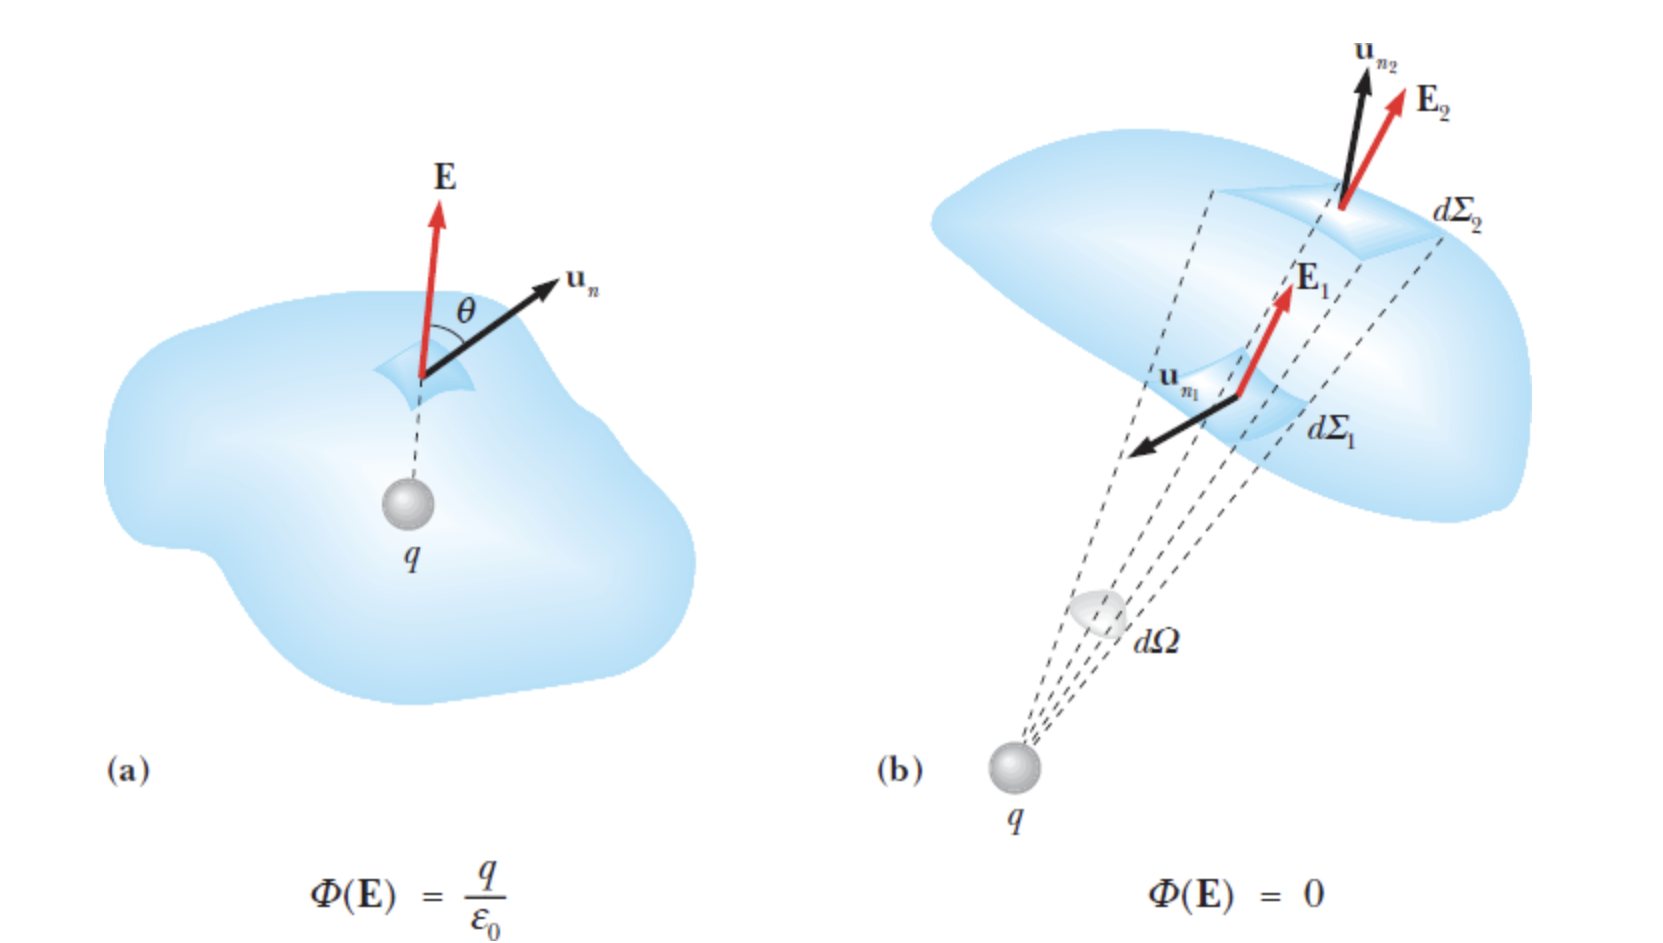
\includegraphics[width=01.0\linewidth]{figure/image8.png}
    \caption{Flusso del campo elettrostatico di una carica puntiforme attraverso una superficie chiusa quando la carica è all'interno della superficie (\textbf{a}) e quando è all'esterno (\textbf{b})}
    \label{fig:chapter_3_3}
\end{figure}

Integrando su tutta la superficie chiusa otteniamo infine 

\begin{equation*}
    \Phi(\mathbf{E}) = \oint_{\Sigma} \mathbf{E} \cdot \mathbf{u}_n \ d\Sigma = 0
\end{equation*}

Questi risultati si possono riassumere dicendo che il flusso attraverso una superficie chiusa del campo elettrostatico di una carica puntiforme $q$ vale $q/\varepsilon_0$ se la carica è interna alla superficie, vale zero se la carica è esterna. 

\newpage

Il risultato enunciato si estende al caso di più cariche puntiformi, attraverso il principio di sovrapposizione e la proprietà di additività dell'integrale.

\begin{equation*}
    \Phi(\mathbf{E}) = \oint_{\Sigma} \mathbf{E} \cdot \mathbf{u}_n  \ d \Sigma = \oint_{\Sigma} (\sum_i \mathbf{E}_i) \cdot \mathbf{u}_n  \ d \Sigma = \sum_i \oint_{\Sigma} \mathbf{E}_i \cdot \mathbf{u}_n  \ d \Sigma
\end{equation*}

Ciascuno integrale vale $q_i/ \varepsilon_0$ se la carica è contenuta all'interno della superficie e vale zero se è esterna. Pertanto abbiamo

\begin{equation*}
    \phi(\mathbf{E}) = \frac{(\sum_i q_i)_{\text{int}}}{\varepsilon_0}
\end{equation*}

Che è esattamente quello che volevamo dimostrare. \\

La legge di Gauss ha delle applicazioni e conseguenze importantissime e si consiglia al lettore di approfondire leggendo tale argomento in \cite{ElettromagnetismoeOnde}
